\section{Experimental Evaluation}
\label{sec:exp}

In order to demonstrate the efficacy of our history-inclusion based
approximation to observational refinement, we argue that our $k$-approximation:
\begin{itemize}

  \item uncovers violations with small values of $k$, and

  \item can be efficiently implemented.

\end{itemize}

To argue both points, we have studied the Scal High-Performance
Multicore-Scalable Computing suite of concurrent data structure
implementations\footnote{\url{http://scal.cs.uni-salzburg.at}} which include
both LIFO- and FIFO-based container objects. Some of these objects, such as the
Michael-Scott Queue~\cite{conf/podc/MichaelS96}, are meant to preserve
observational refinement\footnote{More precisely, they have been designed to be
linearizable.}, while others, such as Kirsch et al.'s
$k$-FIFO~\cite{conf/pact/KirschLP13}, are meant to preserve weaker properties.
For our experiments we have used Scal's C++ implementations without
modification, except to annotate methods with a fixed set of possible
preemption points, e.g.,~preceding accesses to shared storage.

To make the following comparisons, we have developed a tool for enumerating a
(possibly large) number of alternate executions involving a limited number of
object method invocations. We execute each operation on a separate thread, and
ensure that all thread schedules up to a given number $n \in \<Nats>$ of thread
preemptions (at specified preemption points) are executed, similarly to
Microsoft's Chess tool~\cite{conf/osdi/MusuvathiQBBNN08}. With $n=0$
preemptions, there is only one schedule/execution, though the number of
schedules/executions grows exponentially as $n$ increases. For instance, with
our annotation of preemptions in Scal's Michael-Scott Queue, increasing
$n=1..5$ yields $33$, $612$, $8343$, $95434$, and $930141$ schedules, which are
executed at a rate of roughly one million schedules per minute on a MacBook Pro
2.6GHz Intel Core i5 machine.


\subsection{Coverage of Violations}

To show that most violations to observational refinement are uncovered by our
history inclusion approximation for small values of $k$, we measure the number
of violations detected by a traditional linearizability checker versus those
detected by operation counting. On the one hand, the linearizability checker
detects exactly those histories $H(e)$ for which $H(e) \not\in H(L)$, due to
the equivalence of Section~\ref{sec:lin}. On the other hand, operation counting
generally provides lower fidelity: for a given $k \in \<Nats>$, one only
observes the approximation $A_k(H(e)) \preceq H(e)$, unable to resolve $H(e)$
precisely as the number of operations in $H(e)$ exceeds $k$. Thus it cannot be
the case that operation counting detects all histories which violate
observational refinement, for any fixed $k \in \<Nats>$. However, it is
theoretically possible that any given violation $H(e) \not\in H(L)$ of a
certain object could be detected by considering the approximate history
$A_k(H(e'))$ of an alternate execution $e'$ for certain $k$; that is to say
that $A_k(H(e')) \preceq H(e)$, and $A_k(H(e')) \not\in H(L)$. The interesting
empirical question is thus: for varying values of $k \in \<Nats>$, how many
violating histories $H(e)$ are ``covered'' by such an $A_k(H(e'))$?

Figure~\ref{fig:data:coverage} demonstrates that small values of $k$ suffice
for detecting violations. While $k=4$ suffices to cover all violations at
nearly all data points --- besides the first point, where the sample size of
executions is small relative to the number of operations --- all values $k > 0$
capture a nontrivial and increasing number of violations. In fact, as that
sample size increases (the x-axis is ordered by number of executions over
number of operations) the value of $k$ required to capture a violation appears
to decrease, all violations being captured by $k=3$ after a certain point. Note
that this data set only exhibits \emph{order violations} for a FIFO-based
container object, i.e.,~where elements are removed out of order; in general,
there is no cutoff value of $k \in \<Nats>$ for which all violations of such an
object can be captured; see Section~\ref{sec:containers}.

\begin{figure}
  \centering
  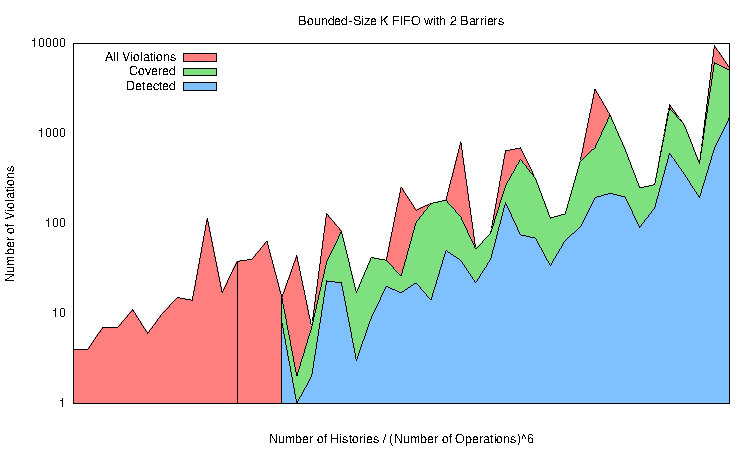
\includegraphics[width=\linewidth]{figures/coverage-bkq-2-barriers}
  \caption{Comparison of observational refinement violations detected with
    $k = 0..4$.
    Each data point measures histories on a logarithmic scale over all
    executions up to $5$ preemptions on Scal's nonblocking bounded-reordering
    queue with $i$ enqueue operations and $j$ dequeue operations.
    The x-axis is ordered by increasing number of executions over $(i+j)$,
    for $i$ and $j$ ranging over $1..4$, and only points with over $1000$
    executions are shown.
    The largest data points measure the total number of unique histories
    encountered over a given set of executions; second are the number of
    those histories which violate linearizability. Next are the number of
    those violations for which weaker histories $A_k(H(e))$ are detected
    for varying values of $k$.
  }
  \label{fig:data:coverage}
\end{figure}

\subsection{Efficiency}

Figure~\ref{fig:data:runtime} compares the runtime overhead of our
operation-counting instrumentation for $k=2$, versus a linearization-based
instrumentation, sampling executions with up to $20$ operations on Scal's
nonblocking Michael-Scott queue $L_\mathrm{msq}$. Since computing the set of
sequential histories $\ker H(L_\mathrm{msq})$ over $n$ operations becomes
prohibitively expensive as $n$ increases --- already surpassing a timeout of
$5$m for $n=7$ --- our measurements bypass the computation of $\ker
H(L_\mathrm{msq})$ entirely, and simply enumerate the linearizations of $H(e)$
for each execution $e$ without checking their inclusion $\ker
H(L_\mathrm{msq})$. Despite our best-effort-efficiency implementation of this
enumeration, one observes the cost incurred by this exponential-time algorithm:
as the number of operations increases --- thus exponentially increasing the
number linearizations --- performance plummets. With only 20 operations,
instrumentation overhead is nearly 100,000\%. Operation counting avoids this
dramatic overhead; though we have not optimized our implementation, we observe
that runtime overhead stays within 30\%.

\begin{figure}
  \centering
  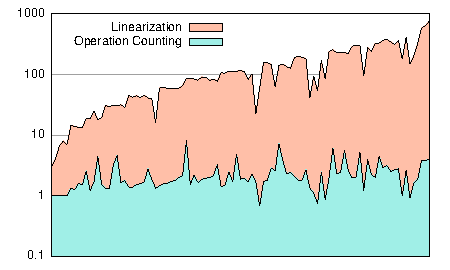
\includegraphics[width=\linewidth]{figures/lin-vs-counting-time}
  \caption{Comparison of runtime overhead between linearization-based monitoring
    and operation counting ($k=2$) for up to $20$ operations. Each data point
    measures runtime on a logarithmic scale, normalized to unmonitored
    execution time, over all executions up to $3$ preemptions on Scal's
    nonblocking Michael-Scott queue with $i$ enqueue operations and $j$ dequeue
    operations. The x-axis is ordered by increasing $i+j$, for $i$ and $j$
    ranging over $1..10$. Times do not include pre-calculation of sequential
    histories for linearization-based monitoring.
  }
  \label{fig:data:runtime}
\end{figure}
